\begingroup
\raggedbottom
\clubpenalty=10000
\widowpenalty=10000
\chapter{Reliability: Bias, Robustness, Privacy, and Safety}
\label{ch:reliability}

A course-support assistant can answer most routine questions correctly while giving unsupported advice on a rare, consequential request. A pedestrian detector can perform well in daylight while missing people in glare. Neither aggregate score describes who encounters the failures, what happens when conditions change, or what the system exposes about its training data.

Reliability connects those questions to evidence about a complete procedure. Data collection, annotation, fitting, thresholds, human review, storage, and actions all affect the result. A written argument can clarify that evidence, but writing it down does not bound a failure probability. A statistical or mathematical bound needs stated assumptions; an operational safeguard needs evidence that it works in the relevant setting.

The support assistant and camera system below are hypothetical teaching cases. Their small numerical examples are constructed, separately from the cited empirical studies. Bias, robustness, privacy, and safety concern different quantities, so the unit and scope of each claim will matter.

\section{Who Receives the Errors?}

Bias can enter through measurement as well as representation. A dataset may omit some language varieties, an annotation rule may mistake a dialect for an error, or a camera may measure some conditions poorly. A loss can reward the most frequent cases while giving little weight to consequential rare ones. A threshold or review queue can then distribute the remaining errors unevenly. This pipeline view is consistent with the sources of harm described by \citet{suresh2021}.

The consequence determines which comparison is useful. \emph{Allocation harm} concerns access to opportunities or resources. \emph{Quality-of-service harm} concerns the accuracy, clarity, or availability of assistance. \emph{Representation harm} concerns categories or descriptions that erase or stereotype people. These can overlap with privacy exposure and physical or operational harm. A single numerical fairness criterion does not decide whether the complete arrangement is acceptable.

\par\noindent\begin{minipage}{\linewidth}
For a fixed predictor $f$ and a nonnegative loss, define population risk and group risk by
\[
R=\mathbb E[\ell(Y,f(X))],\qquad
R_g=\mathbb E[\ell(Y,f(X))\mid G=g],
\]
\end{minipage}\par\addvspace{\belowdisplayskip}
where the relevant group has positive probability. For a finite, disjoint, exhaustive partition, total expectation gives
\[
R=\sum_g P(G=g)R_g.
\]
A group comprising $1\%$ of cases with error $.50$, alongside $99\%$ with error $.01$, produces overall error $.0149$. Overall success is $98.51\%$ while success in the rare group is $50\%$. The average is arithmetically correct; the deployment claim may still be inadequate.

A \emph{slice} is a subset defined by an attribute or condition. Language variety, message length, weather, and pedestrian age can define useful slices. They can overlap, so adding their counts or averaging their rates as if they partitioned the population is generally invalid. Even with a partition, the evaluation proportions may differ from deployment proportions. State the sampling and weighting scheme before interpreting the average.

\par\addvspace{\intextsep}\noindent\begin{minipage}{\linewidth}
\centering
\begin{tikzpicture}[ml diagram, x=1cm, y=1cm]
\node[font=\sffamily\small\bfseries, anchor=west] at (0,.55) {Question};
\node[font=\sffamily\small\bfseries] at (4,.55) {Evidence};
\node[font=\sffamily\small\bfseries] at (7.5,.55) {Scope};
\draw[draw=mlLine] (0,.24) -- (9,.24);
\foreach \y/\theme/\evidence/\claimlimit in {
0/Bias/Group outcomes/Population and labels,
-.72/Robustness/Shift tests or certificate/Specified changes,
-1.44/Privacy/Release accounting/Protected contribution,
-2.16/Safety/Complete action outcomes/Operating conditions}{
  \node[anchor=west, font=\sffamily\small, text=mlAccent] at (0,\y) {\theme};
  \node[font=\sffamily\footnotesize, align=center, text width=3cm] at (4,\y) {\evidence};
  \node[font=\sffamily\footnotesize, align=center, text width=3cm] at (7.5,\y) {\claimlimit};
  \draw[draw=mlLine, line width=.4pt] (0,\y-.35) -- (9,\y-.35);
}
\end{tikzpicture}

\captionof{figure}{Different reliability claims require different evidence and have different limits. Each row connects a question to its scope; it does not certify the complete system.}
\label{fig:reliability-matrix}
\end{minipage}\par\addvspace{\intextsep}

\subsection{Counts, Denominators, and Severity}

A subgroup dashboard can show success, escalation, and severe failures together. Table~\ref{tab:subgroup-dashboard-example} uses integer counts under a fixed rubric: a successful response either answers correctly within authority or routes correctly when required. The slices can overlap. The last column counts adjudicated severe failures, rather than treating every unsuccessful response as equally consequential.

\par\addvspace{\intextsep}\noindent\begin{minipage}{\linewidth}
\centering\small
\setlength{\tabcolsep}{4pt}
\begin{tabular}{@{}L{2.6cm}L{.7cm}L{2.1cm}L{2.1cm}L{1.4cm}@{}}
\toprule
Slice & $n$ & Successful responses & Escalations & Severe failures \\
\midrule
Routine policy & 400 & $364/400=.91$ & $72/400=.18$ & 0 \\
Multilingual phrasing & 70 & $52/70\approx.743$ & $30/70\approx.429$ & 2 \\
Authority-related requests & 45 & $28/45\approx.622$ & $36/45=.80$ & 5 \\
\bottomrule
\end{tabular}
\captionof{table}{A constructed dashboard with explicit denominators. Frequent escalation can coexist with wrong routing or severe failures. Overlapping slices cannot be pooled by summing these rows.}
\label{tab:subgroup-dashboard-example}
\end{minipage}\par\addvspace{\intextsep}

The escalation rate alone does not measure whether escalation was appropriate, reached the right person, or produced a timely resolution. Report those outcomes separately. Small denominators also matter: one changed outcome moves a rate based on $45$ cases by about $2.22$ percentage points. A large observed gap warrants investigation; neither a large nor a small gap establishes a population difference without a suitable sampling and uncertainty analysis. Repeatedly searching slices can also select unusually bad estimates by chance.

Empirical studies can identify problems that averages conceal. Gender Shades evaluated commercial systems on a binary gender-classification task and reported substantial intersectional error disparities \citep{buolamwini2018}. That evidence concerns the evaluated systems, categories, and sample. It supports examining subgroup behavior without making the benchmark's categories a universal definition of identity.

\subsection{Which Binary Errors Matter?}

Let $Y=1$ mean that a message requires escalation and $\hat Y=1$ mean that the assistant escalates it. Constructed confusion counts are
\[
\begin{array}{c|rrrr}
 &\mathrm{TP}&\mathrm{FN}&\mathrm{FP}&\mathrm{TN}\\\hline
A&45&5&10&40\\
B&8&12&2&18
\end{array}
\]
Accuracy is $.85$ for A and $.65$ for B. Combined accuracy is $111/140\approx.793$, but this combines groups with different sample sizes. Conditional rates reveal the missed-escalation problem:
\[
\begin{aligned}
\mathrm{TPR}_A&=45/50=.90,&\mathrm{TPR}_B&=8/20=.40,\\
\mathrm{FPR}_A&=10/50=.20,&\mathrm{FPR}_B&=2/20=.10.
\end{aligned}
\]
The positive predictive values are $45/55\approx.818$ and $8/10=.80$. Similar precision does not imply similar recall: B misses $60\%$ of messages requiring escalation. These rates require nonzero denominators and reliable reference labels. If the labels omit some legitimate escalation needs, equality against those labels does not establish equal service.

\subsection{Requirements Can Conflict}

\emph{Demographic parity} asks for equal positive-prediction rates across groups. \emph{Equalized odds} asks for equal true positive and false positive rates; \emph{equal opportunity} retains the true positive condition \citep{hardt2016}. These are statistical properties of the joint distribution of group, label, and prediction. They do not themselves establish that the labels are appropriate or that a particular causal pathway is absent.

For a group with base rate $\pi_g=P(Y=1\mid G=g)$ in $(0,1)$, total probability gives
\[
q_g=P(\hat Y=1\mid G=g)
=t_g\pi_g+f_g(1-\pi_g),
\]
where $t_g$ and $f_g$ are its true positive and false positive rates. If equalized odds holds with common values $t,f$, then
\[
q_A-q_B=(t-f)(\pi_A-\pi_B).
\]
Thus, with unequal base rates, demographic parity and equalized odds can both hold only if $t=f$. Predicting everyone positive or everyone negative are examples, but the condition also permits random predictions with no class discrimination within either group. When $t=.80,f=0$ and base rates are $.40,.20$, positive-prediction rates are $.32,.16$ despite equalized odds.

A related distinction concerns precision. With $t=.80,f=.10$ at those same base rates, the positive-prediction rates are $.38,.24$, and
\[
\begin{aligned}
P(Y=1\mid\hat Y=1,G=A)&=\frac{.32}{.38}=\frac{16}{19},\\
P(Y=1\mid\hat Y=1,G=B)&=\frac{.16}{.24}=\frac23.
\end{aligned}
\]
Equalized odds therefore need not give equal precision. This example concerns a binary decision; calibration of a continuous probability score is a different property. Specify the property, population, and label meaning rather than referring to an unrestricted impossibility of ``fairness.''

Collecting better data may improve representation or labels. Adjusting thresholds changes an operating point and can trade missed escalations for unnecessary ones. Neither automatically repairs the other problem, and a threshold that helps one rate can worsen another. Observed disparities also do not identify their cause. A causal claim about changing an attribute needs a meaningful intervention or counterfactual model and identification assumptions, as in Chapter~\ref{ch:experiments-claims}; merely holding recorded features fixed is not a causal experiment.

\subsection{Confidence and Information}

For a reported event probability $P$, population calibration means
\[
\mathbb E[Y\mid P]=P.
\]
Group calibration additionally requires $\mathbb E[Y\mid P,G]=P$ where those conditional distributions are defined. A global calibration result need not imply the group property. Confidence $.9$ associated with correctness $.90$ in one group and $.65$ in another gives very different automation risks at the same threshold. Calibration of a classification event also does not calibrate the probability that every sentence in a generated answer is supported.

Calibration is not sufficient for informativeness. Consider equally sized groups with event probabilities $.2$ and $.8$. Predictor A reports those respective probabilities. Predictor B reports $.5$ for everyone. Both are globally calibrated, because B's sole score corresponds to overall prevalence $.5$. B is not calibrated within either group. For a constant prediction $p$ in a group with prevalence $\pi$,
\[
\mathbb E[(p-Y)^2\mid G]
=\pi(1-\pi)+(p-\pi)^2.
\]
A has expected Brier score $.16$; B has $.25$. A uses group information to give sharper correct probabilities. B's calibration alone does not recover that information. Conversely, an informative score can need calibration before it is used for decisions. \citet{guo2017} studied miscalibration and postprocessing in specified neural-classification settings; the evidence does not establish that every neural model has the same calibration error.

\section{What Changes at Deployment?}

Robustness concerns performance under specified changes. A useful statement names a reference distribution $P$, changed distributions $Q$, the measured loss, and the admissible conditions. A clean held-out score estimates risk under its evaluation population, rather than risk under every possible $Q$.

Strict \emph{covariate shift} means that $P(X)$ changes while $P(Y\mid X)$ is preserved on the relevant support. A new camera or different phrasing does not automatically satisfy that condition: measurement changes can alter the conditional relationship too. \emph{Label shift} holds the class-conditional input distribution fixed while changing class prevalence. \emph{Concept drift} concerns a changed predictive conditional distribution; the intended task may remain the same. A policy change can instead change the target definition itself. Diagnose which assumption is being invoked before choosing a correction.

Shortcut use is one possible source of shift failure. A predictor may use a source marker, background, or document format that correlates with the label in development data but changes elsewhere. The association may be highly predictive in the original population. Calling it a shortcut states a concern about the intended task and transfer, rather than proving that it is statistically useless.

The chest-radiograph study by \citet{zech2018} varied pneumonia prevalence across hospital-source training subsets and compared internal with external evaluation. Figure~\ref{fig:zech-domain-shift} shows that stronger internal performance can coexist with weaker external performance as the source association changes. The experiment supports concern about source-dependent generalization; the plotted curves alone do not uniquely identify the particular visual cue used by the model.

\par\addvspace{\intextsep}\noindent\begin{minipage}{\linewidth}
\centering
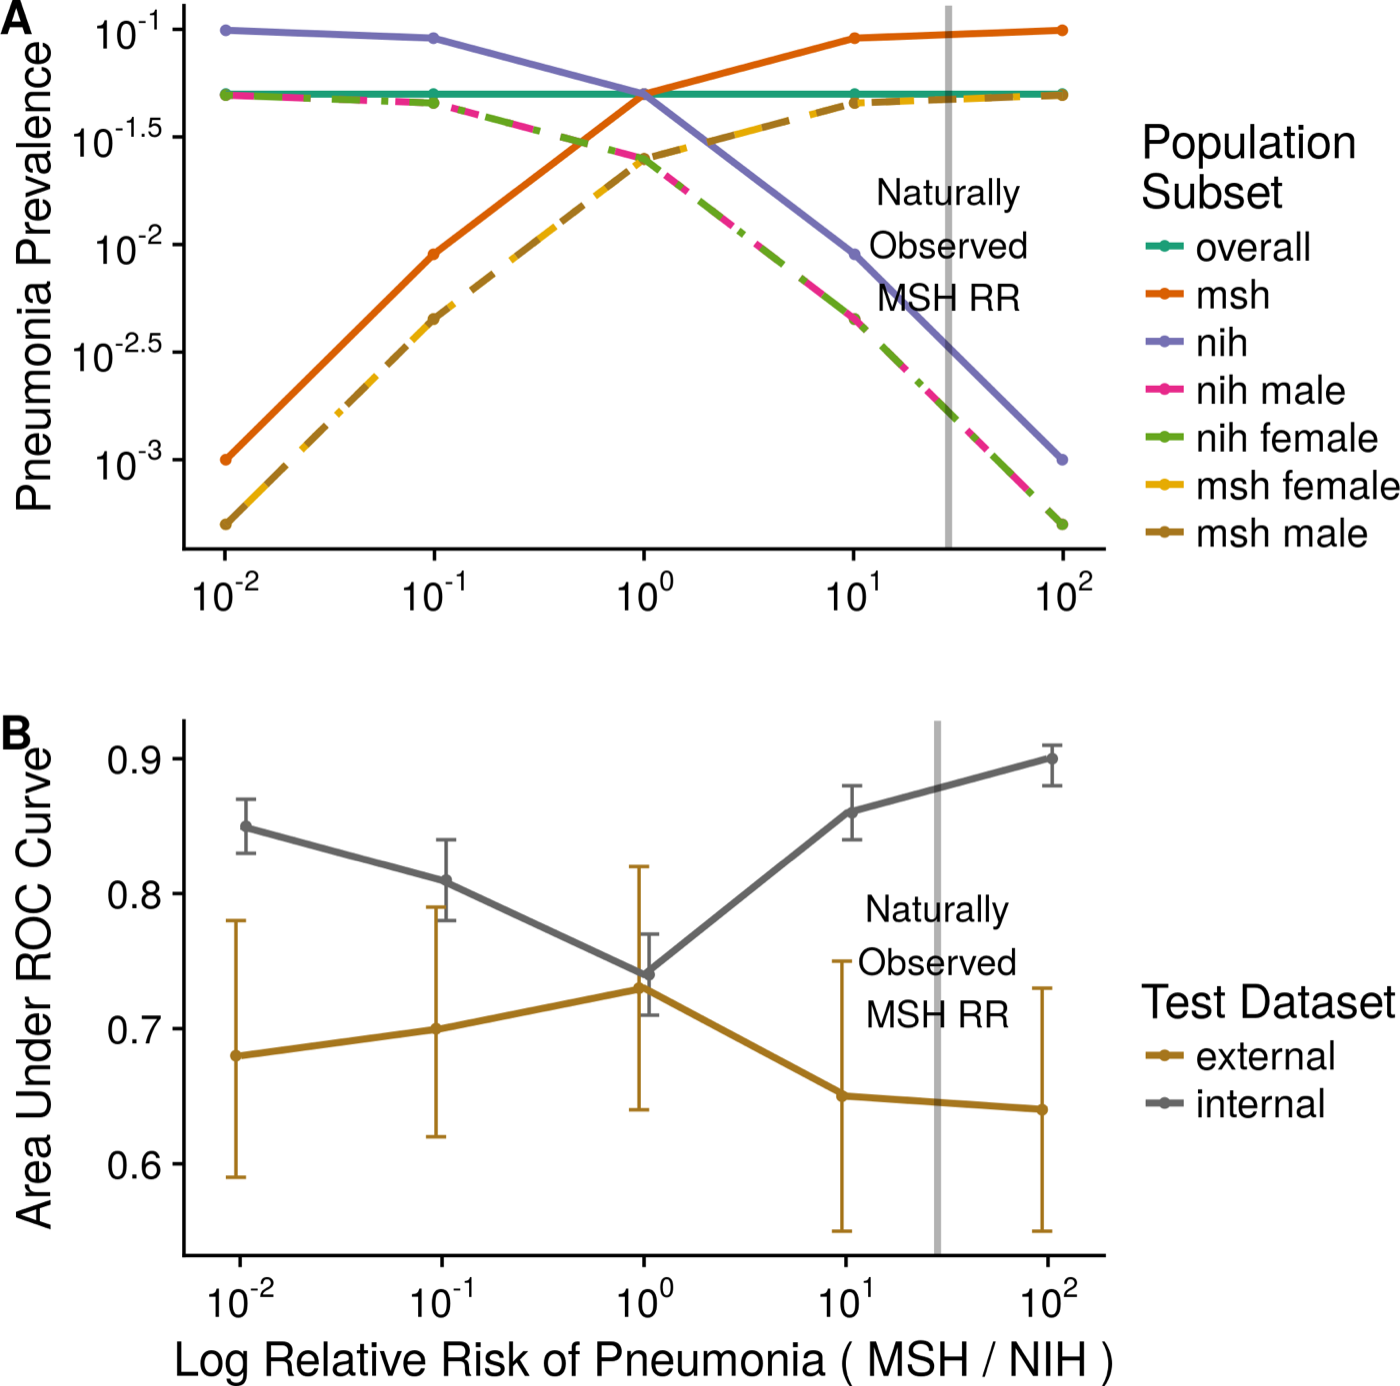
\includegraphics[width=.78\linewidth]{figures/external/zech2018_g003_small.png}
\captionof{figure}{Engineered pneumonia prevalence by source (A) and ROC AUC (B) in the experiment of \citet{zech2018}. Internal testing uses held-out MSH--NIH cases; external testing uses Indiana University cases. Bars show $95\%$ confidence intervals. The horizontal coordinate is the MSH/NIH prevalence ratio on a logarithmic scale. MSH denotes Mount Sinai Hospital; NIH denotes the NIH ChestXray source. Reproduced from the PLOS Medicine article under CC BY 4.0.}
\label{fig:zech-domain-shift}
\end{minipage}\par\addvspace{\intextsep}

A constructed assistant comparison illustrates a narrower claim. Mean familiar-wording success falls from $.914$ to $.892$ after paraphrase augmentation and query rewriting, while shifted-wording success rises from $.627$ to $.812$. The changes are $-.022$ and $+.185$: a tradeoff between the two specified conditions. These means alone do not give uncertainty, identify which component caused the change, or establish robustness to other institutions or policy updates.

\par\addvspace{\intextsep}\noindent\begin{minipage}{\linewidth}
\centering\small
\begin{tabular}{@{}L{2.4cm}L{3.3cm}L{4cm}@{}}
\toprule
System & Specified change & Outcome to measure \\
\midrule
Support assistant & Paraphrase or language variety & Correct routing and supported answers \\
Support assistant & Policy-page revision & Retrieval of current evidence and stale claims \\
Pedestrian detector & Night rain or camera placement & Condition-specific misses and latency \\
Forecasting system & Delayed sensor reports & Error over the affected horizon \\
\bottomrule
\end{tabular}
\captionof{table}{Stress tests connect a deployment change to an outcome. Common-corruption benchmarks provide repeatable additional probes \citep{hendrycks2019}; their coverage does not encompass every realistic shift.}
\label{tab:reliability-stress-tests}
\end{minipage}\par\addvspace{\intextsep}

Geometric image tests must transform detection or segmentation labels consistently. Language paraphrases must preserve the relevant request and policy meaning. A change that alters the true answer is not a label-preserving robustness test. After a failed stress test guides a revision, that test has become development evidence; a fresh protected evaluation is needed for the revised procedure's claim.

\subsection{Adversarial Risk and Certificates}

An adversary chooses changes deliberately. Specify the access, budget, valid input domain, and success criterion. For a perturbation set $\mathcal A(x)$ whose intended label remains $y$, an adversarial-training objective is
\[
\min_\theta\;\mathbb E\!\left[
\sup_{\delta\in\mathcal A(X)}
\ell(Y,f_\theta(X+\delta))\right].
\]
A norm ball can define $\mathcal A(x)$, intersected with valid inputs. Projected-gradient attacks approximate this inner optimization \citep{madry2018towards}; finding one damaging perturbation establishes vulnerability, while failing to find one does not prove that the supremum is small. For zero-one loss, accuracy against a particular attack is an upper bound on accuracy against the full permitted adversary, provided the attack's outputs stay in that set.

For class-probability vector $p_\theta(x)$, a TRADES-style surrogate instead combines clean prediction with local consistency \citep{zhang2019trades}:
\[
\begin{aligned}
J(\theta)&=\mathbb E[\ell(Y,p_\theta(X))]\\
&\quad+\lambda\,\mathbb E\!\left[
\sup_{\delta\in\mathcal A(X)}
\mathrm{KL}\bigl(p_\theta(X)\|p_\theta(X+\delta)\bigr)\right].
\end{aligned}
\]
Here $\lambda\ge0$ uses the reciprocal convention of the original paper. Larger $\lambda$ weights consistency more heavily; it does not guarantee a particular fitted robustness or clean accuracy. The consistency loss and worst-case label loss are different objectives.

A certificate needs a verified bound rather than a successful attack search. Suppose every class score $f_j$ is $L$-Lipschitz in the $\ell_2$ norm on a region containing the permitted ball, with $L>0$. At $x$, let $y$ be the uniquely highest-scoring class and
\[
m=f_y(x)-\max_{j\ne y}f_j(x)>0.
\]
For each competing $j$ and $\|\delta\|_2\le r$, the score difference satisfies
\[
f_y(x+\delta)-f_j(x+\delta)
\ge f_y(x)-f_j(x)-2Lr\ge m-2Lr.
\]
Therefore $r<m/(2L)$ certifies an unchanged class. With $m=.6,L=3$, every permitted perturbation with norm strictly below $.1$ is covered; equality can permit a tie. This certifies agreement with the original prediction, not that the prediction was correct.

A vector-valued $L$-Lipschitz bound also implies the per-score bound and hence this conservative radius. Products of valid operator-norm bounds and activation Lipschitz bounds can control a simple sequential network, but the calculation must cover every operation, including residual paths or normalization. A few sampled input pairs give a lower estimate of possible variation, not a global upper bound. A certificate for one ball does not transfer to a physical or semantic change outside it.

\section{What Can a Release Reveal?}

Privacy concerns the information available to particular observers through particular paths. A support message can expose sensitive circumstances through prompts, logs, annotation exports, or retrieval indexes even if the final answer omits a name. Camera footage can identify or link people through faces, clothing, locations, and trajectories. Discarding raw frames may reduce exposure while retained trajectories remain linkable. Blurring and redaction are useful controls whose sufficiency depends on the observer and auxiliary information.

\par\addvspace{\intextsep}\noindent\begin{minipage}{\linewidth}
\centering\small
\begin{tabular}{@{}L{2.4cm}L{2cm}L{2.2cm}L{3.1cm}@{}}
\toprule
Asset & Observer & Access path & Control and remaining question \\
\midrule
Sensitive student disclosure & Unassigned staff & Debugging logs & Restrict access and retention; inspect exports \\
Identity and grades & Compromised account & Retrieval index & Limit privileges; test accessible records \\
Bystander identity or trajectory & Later data user & Video or metadata & Reduce retained detail; assess linkage \\
\bottomrule
\end{tabular}
\captionof{table}{A threat model connects an asset, observer, and access path. A control addresses a specified exposure rather than making every downstream use private.}
\label{tab:privacy-threat-model-example}
\end{minipage}\par\addvspace{\intextsep}

Data minimization, access controls, retention limits, and secure storage can reduce direct exposure. Federated learning keeps raw data decentralized in some workflows, but transmitted updates can still reveal information. Filtering a model's outputs or keeping data on devices does not by itself establish a formal privacy guarantee. The privacy analysis must cover the releases and the data path actually accessible to the observer.

\subsection{Differential Privacy Defines a Contribution}

Choose an adjacency relation $D\sim D'$ describing the contribution to protect. Adding or removing one record is one choice; replacing one record in a fixed-size dataset is another. Protecting a person who contributes many records requires a person-level relation or an accounting argument for those records.

A randomized mechanism $M$ is $(\epsilon,\delta)$-differentially private, with $\epsilon\ge0$ and $0\le\delta<1$, if, for every neighboring pair and every measurable output event $S$,
\[
P(M(D)\in S)\le e^\epsilon P(M(D')\in S)+\delta.
\]
Adjacency is symmetric, so the condition also applies with $D,D'$ reversed \citep{dwork2006,dwork2014privacy}. Pure DP has $\delta=0$. Smaller $\epsilon$ restricts the permitted distinction more strongly; $\delta$ is additive slack in an event-probability bound, not generally an independent probability that an entire run ``fails.''

DP limits the evidence a release supplies for distinguishing neighboring datasets. It allows population information to be learned and does not prevent an observer from correctly guessing a fact already predictable from other evidence. If the mechanism protects one record, calling its output ``person-private'' without controlling a person's contributions changes the claim. For pure DP, chaining at most $k$ record changes gives the weaker bound $k\epsilon$ by multiplying the inequalities.

\subsection{Sensitivity and Noise}

For a vector query $q$, define sensitivity under the chosen adjacency by
\[
\Delta_1=\sup_{D\sim D'}\|q(D)-q(D')\|_1.
\]
For $\epsilon>0$ and finite positive $\Delta_1$, release $q(D)$ plus independent Laplace noise in each coordinate with scale $b=\Delta_1/\epsilon$. At any output $z$, the density ratio is
\[
\frac{p_D(z)}{p_{D'}(z)}
=\exp\!\left(\frac{\|z-q(D')\|_1-\|z-q(D)\|_1}{b}\right)
\le e^{\Delta_1/b}=e^\epsilon.
\]
The triangle inequality supplies the bound; integrating over events proves pure DP. A zero-sensitivity query is constant on adjacent datasets and needs no noise for that guarantee.

For a fixed-size sample of $n=100$ values clipped to $[0,1]$, under \emph{replacement} adjacency, the mean has sensitivity $1/100$. With $\epsilon=.5$, noise scale is $.02$. Laplace noise has mean zero, expected absolute magnitude $b=.02$, and variance $2b^2=.0008$. The original sampling error remains; these quantities describe the additional mechanism noise. The sensitivity changes if the protected unit or contribution bounds change.

Gaussian noise uses $\Delta_2=\sup_{D\sim D'}\|q(D)-q(D')\|_2$. A classical sufficient condition, for $0<\epsilon<1$ and $0<\delta<1$, adds independent zero-mean Gaussian noise per coordinate with standard deviation
\[
\sigma>\frac{\Delta_2\sqrt{2\log(1.25/\delta)}}{\epsilon}
\]
\citep{dwork2014privacy}. This is a sufficient calibration with a restricted range, rather than an equality giving the best possible noise for every budget.

DP-SGD bounds each example's gradient before adding noise \citep{abadi2016}. For clipping norm $C>0$,
\[
\tilde g_i=\frac{g_i}{\max(1,\|g_i\|_2/C)},\qquad
\|\tilde g_i\|_2\le C.
\]
For the clipped sum, replacing one contribution changes it by at most $2C$; adding or removing one changes it by at most $C$. Noise, sampling, normalization, and the accountant must match the selected adjacency and training mechanism. Clipping alone only bounds influence; it does not make an unnoised release DP.

\subsection{Several Releases and an Observer's Accuracy}

Basic adaptive composition gives total parameters $(\sum_j\epsilon_j,\sum_j\delta_j)$ when each release is $(\epsilon_j,\delta_j)$-DP conditional on each possible preceding transcript. Postprocessing a private release without additional access to the private dataset preserves its guarantee \citep{dwork2014privacy}. Publishing more independently noised queries consumes more budget; simply transforming an already released value does not. More refined accountants can improve basic bounds under their stated conditions. They do not universally replace $k\epsilon$ by $\sqrt{k}\epsilon$.

Hyperparameter search, private-data validation, and additional released summaries can also contribute privacy cost. Calling the final fit DP while ignoring these accesses can omit part of the release mechanism. Conversely, separately releasing raw training data is not repaired by making the model private.

A precise testing example makes the direction of the guarantee visible. Suppose two fixed neighboring datasets have equal prior probability. Let their output distributions be $P,Q$ under a pure $\epsilon$-DP mechanism, and write $t=e^\epsilon$. For an event $A$ with $d=P(A)-Q(A)\ge0$, applying DP to $A$ and to its complement gives
\[
d\le(t-1)Q(A),\qquad
d\le\frac{t-1}{t}(1-Q(A)).
\]
Their largest joint upper bound is $(t-1)/(t+1)$. Taking the supremum over events bounds total variation. An optimal equal-prior test consequently has accuracy and excess accuracy bounded by
\[
\operatorname{Acc}\le\frac12+
\frac{e^\epsilon-1}{2(e^\epsilon+1)},\qquad
\operatorname{Adv}_{\mathrm{acc}}\le\frac12\tanh(\epsilon/2).
\]
For $\epsilon=.1,1,5$, the excess bounds are approximately $.025,.231,.493$. Increasing $\epsilon$ weakens protection. These are upper bounds for this neighboring-dataset experiment, not predictions of an observed attack's success or bounds for an arbitrary membership experiment with a different prior and data construction.

Membership-inference attacks try to identify whether a candidate contributed to fitting. Shadow-model attacks studied by \citet{shokri2017} exploit output differences between included and held-out examples. Their measured accuracy concerns a specified attack and experiment. Model inversion, linkage, and access to raw logs pose other questions. A DP claim must identify the release and adjacency; a privacy review must also address direct exposures outside that claim.

\section{What Happens After Deferral?}

Safety concerns consequences of the complete action procedure. A missed close-range pedestrian can matter because of the resulting trajectory, latency, and braking response. An unsupported assistant answer can matter because the user follows it instead of reaching an authorized office. A hazard description connects an error to such a consequence, identifies conditions where it can occur, and supplies evidence for prevention or mitigation.

A fallback must be evaluated as an action. A human reviewer can be unavailable, delayed, or wrong; an automated escalation can reach the wrong destination. In the hypothetical assistant, routing a high-risk message to trained staff may reduce unsupported advice, but the routing, response time, and staff outcome still require measurement. For the camera system, slower operation or takeover may reduce some hazards while introducing others. Neither a confidence threshold nor a written safety case alone supplies a bound on harm.

\subsection{Selective Risk and Complete Risk}

Let $c(x)\in\{0,1\}$ select automated cases, and let $\ell$ denote their nonnegative loss. Population coverage and selective risk are
\[
\phi=\mathbb E[c(X)],\qquad
R_{\mathrm{auto}}=\frac{\mathbb E[c(X)\ell]}{\phi},\quad\phi>0.
\]
On $n$ observations, empirical coverage is $\hat\phi=n^{-1}\sum_i c_i$, and empirical selective risk is $\sum_i c_i\ell_i/\sum_i c_i$ when the denominator is positive. These empirical quantities estimate population ones under an appropriate evaluation design. Selective classification studies this coverage--risk tradeoff \citep{geifman2017}.

For a fixed score $a(x)$, raising a threshold in $c_\tau(x)=\mathbf1\{a(x)\ge\tau\}$ cannot increase coverage. It need not decrease error. With scores $(.99,.95,.90,.85,.70,.55)$ and correctness indicators $(0,1,1,1,0,1)$, threshold $.80$ selects four cases with error $1/4$ and coverage $2/3$. Threshold $.96$ selects one case with error $1$ and coverage $1/6$. The highest-confidence case is wrong.

If $a$ is population-calibrated for correctness, so that $P(\text{correct}\mid a)=a$, selecting solely by $a\ge\tau$ gives expected zero-one selective risk at most $1-\tau$. This statement does not transfer to severity-weighted loss, every group, or every finite sample, and it requires the calibration property in the relevant population.

Use the same loss scale for automated and deferred outcomes. If $R_{\mathrm{defer}}$ is the conditional risk after deferral and $0<\phi<1$, total risk is
\[
R_{\mathrm{complete}}=\phi R_{\mathrm{auto}}
+(1-\phi)R_{\mathrm{defer}}.
\]
At coverage $.8$, automated risk $.01$, and deferred risk $.10$, complete risk is $.028$. Reporting only $.01$ omits the outcomes of one fifth of the cases. Review cost, delay, and unequal access can require additional outcomes beyond this single loss.

\subsection{Rare Failures Need Adequate Evidence}

Zero observed severe failures does not establish zero risk. For $n$ independent cases with common severe-failure probability $p$, the chance of observing no failures is $(1-p)^n$. After zero failures, a one-sided $95\%$ binomial upper confidence bound is
\[
p_{\mathrm{upper}}=1-.05^{1/n}.
\]
At $n=300$, this is about $.00994$, close to the approximation $3/n=.01$. The confidence statement concerns a repeated sampling procedure and its assumptions; it is not a posterior probability that this system's risk lies below the bound. Correlated video frames are not $300$ independent operating episodes, and a routine-case sample does not certify a rare high-risk slice.

A reliability decision may therefore restrict the operating conditions, require further evidence, or decline deployment. Documenting a missing fallback or an unacceptable subgroup outcome makes the limitation concrete. Monitoring can support later decisions, but it does not compensate for an unevaluated hazard at launch.

\section{What Does an Explanation Describe?}
\label{sec:xai-toolkit}

An explanation method answers a chosen question about a fixed predictor and a reference distribution. It may allocate a prediction among features, approximate the predictor locally, summarize average response to feature substitution, or find a change that flips an output. Those questions are distinct from whether a prediction is true, equitable, or caused by a particular real-world mechanism.

\subsection{Attribution Depends on the Reference}

For $d$ features and case $x$, choose a finite-valued coalition function $v(S)$ for subsets of features. SHAP uses Shapley allocations \citep{lundberg2017shap}:
\[
\phi_j=\sum_{S\subseteq\{1,\ldots,d\}\setminus\{j\}}
\frac{|S|!(d-|S|-1)!}{d!}
\bigl[v(S\cup\{j\})-v(S)\bigr].
\]
The allocations satisfy $\sum_j\phi_j=v(\{1,\ldots,d\})-v(\varnothing)$. If the full-coalition value is $f(x)$, they add to the prediction's difference from the baseline. This identity describes the chosen coalition game. It does not remove the need to define what an ``absent'' feature means.

For instance, conditional expectations $v(S)=\mathbb E[f(X)\mid X_S=x_S]$ use associations in the reference population. Substituting $x_S$ while sampling missing coordinates from a marginal reference defines another game and can create unrealistic combinations. Its occasional description as ``interventional'' is not, by itself, a causal identification argument.

Consider $X_1=X_2=Z$ with $P(Z=1)=1/2$, rule $f(x)=x_1$, and case $(1,1)$. The conditional game has values
\[
v(\varnothing)=.5,\quad v(\{1\})=v(\{2\})=v(\{1,2\})=1.
\]
For two features, averaging the two possible addition orders gives $\phi_1=\phi_2=.25$. Feature 2 receives attribution because it reveals feature 1, even though the prediction formula does not use $x_2$. Under marginal substitution, $v(\{2\})=.5$, giving $\phi_1=.5,\phi_2=0$. Both allocations satisfy the addition identity; they describe different references.

\subsection{Approximations and Proposed Changes}

LIME fits a simple surrogate near a case, with a chosen perturbation distribution, distance weighting, and complexity penalty \citep{ribeiro2016lime}. A representative objective is
\[
\min_{g\in\mathcal G}\;
\mathbb E_Z[w_x(Z)(f(Z)-g(Z))^2]+\Omega(g).
\]
The result is an approximation within that sampling and model family. Evaluate its local fidelity on the relevant neighborhood. Small changes in the neighborhood, weighting, or features can change the explanation. Agreement with another method or with an expert can be informative, but is not proof of fidelity or causal truth.

A partial dependence function for feature $j$ averages substitutions:
\[
\mathrm{PD}_j(z)=\mathbb E[f(z,X_{-j})]
\]
under a stated reference distribution. If $X_1=X_2=Z$ as above and $f(x)=x_1-x_2$, all observed predictions are zero, yet $\mathrm{PD}_1(z)=z-.5$. The curve evaluates combinations outside the observed diagonal. It is not the observed effect of changing one real-world feature while everything else remains feasible.

A prediction counterfactual seeks an admissible $x'$ with a changed output, often minimizing a chosen distance or cost. A small change under that cost need not be actionable, lawful, or effective at changing the actual outcome. Constraints must encode feasible changes and their dependencies. A feature-substitution counterfactual also differs from a causal counterfactual about how a person's world would have developed under another intervention.

Gradient or image-saliency explanations similarly require method-specific checks. Model or label randomization can reveal insensitivity to the fitted predictor \citep{adebayo2018sanity}. Masking highlighted regions can itself introduce artifacts. Neither a plausible picture nor its removal experiment uniquely identifies a causal mechanism. Explanation evidence should support a particular audit question alongside outcome and slice evaluation.

\section{Which Uncertainty Guarantee Applies?}
\label{sec:uq-reliability}

Outcome variability and uncertainty about a fitted predictor can both affect decisions, as discussed in Chapter~\ref{ch:probabilistic-models}. An uncertainty signal is useful when evidence connects it to the desired decision outcome. Neither a wide interval nor agreement among models is inherently a safety guarantee.

\subsection{Split Conformal Prediction}

Fix the predictor and a measurable, finite-valued nonconformity score $s(x,y)$ before using calibration observations. Conditional on the training data and fitting randomness, assume the $n$ calibration observations and a fresh test observation are exchangeable: their joint distribution is invariant to permutations. An independent training split followed by i.i.d. calibration and test cases is sufficient. An arbitrary new domain or temporal drift need not satisfy the condition \citep{shafer2008,angelopoulos2023}.

For regression, choose $s(x,y)=|y-\hat f(x)|$; for classification, one option is $s(x,y)=1-\hat p(y\mid x)$. \par\noindent\begin{minipage}{\linewidth}
Sort the calibration scores as $s_{(1)}\le\cdots\le s_{(n)}$. For $0<\alpha<1$, set
\[
k=\lceil(n+1)(1-\alpha)\rceil,\qquad
\hat q=\begin{cases}s_{(k)},&k\le n,\\+\infty,&k=n+1.\end{cases}
\]
\end{minipage}\par\addvspace{\belowdisplayskip}
The prediction set is
\[
\mathcal C(x)=\{y:s(x,y)\le\hat q\}.
\]
This uses an order statistic, not an interpolated percentile. With finite scores, the infinite-threshold convention accepts every candidate.

For scores without ties, exchangeability makes the test score's rank uniform among all $n+1$ scores, conditional on the fitted procedure. Acceptance occurs at rank at most $k$, so
\[
P(Y_{n+1}\in\mathcal C(X_{n+1}))
=\frac{k}{n+1}\ge1-\alpha.
\]
With ties, accepting all boundary ties preserves the lower bound, although coverage can be conservative. The bound averages over both the calibration sample and the fresh case. It is not a guarantee conditional on a particular realized calibration sample, input, or subgroup. Selecting the score or predictor adaptively on the same calibration outcomes can break the argument.

For nine sorted residuals
\[
.1,.2,.2,.3,.4,.5,.7,.9,1.2,
\]
target coverage $.80$ gives $k=8$ and $\hat q=.9$. A point prediction $5$ receives $[4.1,5.9]$. Target $.90$ gives $k=9$, threshold $1.2$, and interval $[3.8,6.2]$. Target $.95$ gives $k=10$ and an unbounded interval. The valid guarantee can be uninformative at a small calibration size.

If residuals are actually independent of input and follow $\mathcal N(0,.3^2)$, their population $90\%$ absolute quantile is $.3\Phi^{-1}(.95)\approx.494$. A large i.i.d. calibration sample tends toward that threshold and width about $.99$. This numerical comparison uses Gaussian residuals; the conformal rank bound does not. A positive scale estimate fixed before calibration permits score $|y-\hat f(x)|/\hat\sigma(x)$ and intervals with half-width $\hat q\hat\sigma(x)$. Varying width alone does not establish exact conditional coverage at every $x$.

\subsection{Coverage and Usefulness Are Distinct}

A classifier reporting $.5$ for each of two labels gives score $.5$ on every case. Calibration then produces a set containing both labels, with coverage one but no discrimination. Reconstruction of a marginal coverage guarantee does not make a weak predictor informative.

Marginal coverage can also conceal group differences. If $90\%$ of the population receives coverage $.98$ and $10\%$ receives coverage $.20$, overall coverage is $.902$. This meets a $.90$ target while serving the rare group poorly. For prespecified groups, calibrating within each group can supply a separate rank bound when the calibration and test cases are exchangeable within that group. Small groups may require infinite thresholds or wide sets. Adaptive widths and group-specific calibration address different problems; neither gives unrestricted guarantees under shift.

Ensemble disagreement is another signal. For $M>1$ probability estimates of one event, a sample spread is
\[
V(x)=\frac1{M-1}\sum_{m=1}^M(p_m(x)-\bar p(x))^2.
\]
\citet{lakshminarayanan2017ensembles} studied deep ensembles empirically in specified uncertainty evaluations. An operational threshold can be chosen on protected development data and evaluated on fresh cases. All members can share a shortcut, be equally overconfident, or agree on a wrong answer; $V(x)=0$ then supplies no error bound. A rising disagreement rate can motivate a shift investigation without proving that the error rate has risen. Outcome labels are needed to test that link.

\section{What Can an Adversary Reach?}
\label{sec:security-reliability}

Security examines deliberate interference with an asset through an accessible surface. Natural-shift tests do not evaluate every motivated adversary. A threat model specifies who can submit queries, modify documents, contribute feedback, inspect outputs, or access infrastructure. The success criterion and the defended scope determine which controls and evaluations are relevant.

Poisoning places adversarial contributions in training or feedback. It can degrade overall performance or create a targeted trigger. Supply-chain attacks can enter through data or pretrained weights; version pinning records what was used but does not establish that it is clean. Adversarial examples instead act on test inputs \citep{szegedy2014,goodfellow2015}. A physical change is covered by a mathematical certificate only if its effect lies within the certificate's specified input set. Its physical origin alone neither places it inside nor outside a norm ball.

Model extraction targets a model's behavior or parameters through queries. Membership inference targets inclusion, while inversion seeks information associated with records or attributes. These assets and experiments differ, so one measured defense should not be treated as covering them all. Rate limits, access controls, release design, and privacy mechanisms address different portions of the surface.

Prompt injection supplies adversarial instructions through user input or content the model was meant to treat as data. Indirect injection can arrive in retrieved documents. \citet{greshake2023indirect} demonstrated compromises in particular language-model-integrated applications; the results establish possible failure paths, rather than a universal attack success rate for every current system.

Separating instruction and data with markers can help a model interpret content but does not impose a security boundary. Sanitization can miss unfamiliar instructions. Enforce tool permissions and authorization outside generated text, limit the accessible data and actions, review document provenance, and evaluate attacks within the stated capabilities. These controls still need evidence and a documented residual scope.

\par\addvspace{\intextsep}\noindent\begin{minipage}{\linewidth}
\centering\small
\begin{tabular}{@{}L{2.1cm}L{7.6cm}@{}}
\toprule
Threat field & Concrete assistant example \\
\midrule
Asset and adversary & Routing integrity; contributor able to edit retrieved pages \\
Surface and success & Retrieval content; unauthorized direct advice or tool action \\
Preventive control & Reviewed index updates and externally enforced permissions \\
Monitoring evidence & Audited unauthorized actions and unmatched document changes \\
Recovery & Disable affected actions and restore a reviewed snapshot \\
Residual scope & Infrastructure compromise needs a separate access-control analysis \\
\bottomrule
\end{tabular}
\captionof{table}{One scoped security threat card. Recovery can limit further exposure; reverting an index does not undo an action or information already disclosed.}
\label{tab:security-threat-card}
\end{minipage}\par\addvspace{\intextsep}

After launch, monitor outcomes tied to the original risks: subgroup routing, delayed reviews, changed policy evidence, condition-specific misses, and unauthorized actions. Input-distribution alarms are proxies rather than direct measurements of correctness. Audits and logs must also respect the privacy design. When evidence changes, narrowing operation, disabling a vulnerable path, or withdrawing the system can be the warranted response.

\begin{studyquestions}
\item How can measurement, labels, loss weighting, and thresholds distribute harm differently?
\item Which assumptions permit aggregate risk to be written as a weighted average of group risks?
\item Why can accuracy, precision, recall, escalation rate, and severe-failure count support different conclusions?
\item Under which conditions do demographic parity and equalized odds conflict?
\item Why are calibration, informativeness, and causal fairness different properties?
\item What distinguishes natural shift, an attack evaluation, and a perturbation certificate?
\item How do adjacency, sensitivity, and composition determine a privacy claim?
\item What can an equal-prior neighboring-dataset test say about privacy, and what remains outside it?
\item Why must a fallback's outcomes enter the complete risk calculation?
\item Which reference and feasibility choices change attribution or prediction counterfactuals?
\item What is exchangeability, and over which randomness does split-conformal coverage average?
\item Why can valid marginal coverage or low ensemble disagreement coexist with poor service?
\item Which attack capabilities can instruction markers, access controls, and reviewed updates actually address?
\end{studyquestions}

\begin{exercises}[Use explicit denominators and distinguish observations from guarantees.]
\item \exercisetag{Calculation}{Core}Design a confusion matrix with nonzero positive and negative counts. Compute its true positive and false positive rates and interpret them for escalation.
\item \exercisetag{Diagnosis}{Core}Construct a subgroup failure hidden by a strong overall score. Specify the group weight and show the aggregation.
\item \exercisetag{Concept}{Core}Describe a plausible shortcut in vision, language, or audio. State a changed condition that would test reliance on it and one alternative explanation for failure.
\item \exercisetag{Concept}{Advanced}Give a privacy design that reduces a particular exposure while reducing measured utility. State the asset, observer, and residual exposure.
\item \exercisetag{Concept}{Intermediate}Describe a task where a predictor should assist a human. Identify a failure in the review path that assistance alone does not rule out.
\item \exercisetag{Diagnosis}{Intermediate}Describe a deployment where specified-shift performance matters more than clean benchmark accuracy. Explain whether strict covariate shift is established.
\item \exercisetag{Diagnosis}{Intermediate}For either running case, name a subgroup, shift, privacy path, and severe hazard. Identify the outcome and sampling unit for each.
\item \exercisetag{Design}{Intermediate}Draft a reliability argument connecting a subgroup failure, hazard, and fallback. State the missing evidence, rather than treating the argument as a certificate.
\item \exercisetag{Design}{Intermediate}Specify aggregate risk, group risk, and a changed population for one predictor. Explain why the first alone need not control either of the others.
\item \exercisetag{Design}{Intermediate}Use Table~\ref{tab:security-threat-card} to describe an attack against a system. Name the asset, adversary, surface, success criterion, control, monitoring evidence, recovery, and residual scope.
\item \exercisetag{Calculation}{Intermediate}Reproduce the two-group calibration example with prevalences $.2,.8$. Compute both Brier scores and distinguish global from group calibration.
\item \exercisetag{Calculation}{Core}For the two escalation confusion matrices, compute overall accuracy, group recall, false positive rate, and precision. Which comparison reveals missed escalations most directly?
\item \exercisetag{Calculation}{Intermediate}For base rates $.4,.2$ and shared TPR $.8$, FPR $.1$, calculate positive-prediction rates and precision. Derive the condition under which demographic parity can coexist with equalized odds.
\item \exercisetag{Calculation}{Intermediate}With score margin $.6$ and a valid per-score Lipschitz bound $L=3$, give the certified open radius. Explain what correctness and equality at the boundary remain unestablished.
\item \exercisetag{Calculation}{Intermediate}For a fixed-size clipped mean of $100$ values in $[0,1]$, use replacement adjacency and $\epsilon=.5$. Compute sensitivity, Laplace scale, expected absolute noise, and noise variance. Repeat the scale if the protected contribution can replace ten records.
\item \exercisetag{Calculation}{Intermediate}Compose three adaptive releases, each $(.2,10^{-6})$-DP under the same adjacency. For pure DP with $\epsilon=\log 3$, compute the equal-prior excess-accuracy bound. Explain why postprocessing a release differs from another private-data query.
\item \exercisetag{Calculation}{Intermediate}Reproduce the six-case threshold example's coverage and selective error at $.80,.96$. With automated coverage $.8$, automated risk $.01$, and deferred risk $.10$, compute complete risk.
\item \exercisetag{Calculation}{Intermediate}For the nine residuals, compute split-conformal ranks, thresholds, and intervals around $5$ at target coverages $.80,.90,.95$. Explain why changing the score after seeing calibration errors needs a new validity argument.
\item \exercisetag{Calculation}{Intermediate}After zero severe failures in $300$ independent identically distributed episodes, compute the one-sided $95\%$ binomial upper bound. Explain what changes when these are consecutive frames of one episode.
\item \exercisetag{Calculation}{Advanced}Compute both two-feature SHAP allocations for the correlated-feature example and the partial dependence curve for $f(x)=x_1-x_2$. Explain their differing questions.
\end{exercises}

\clearpage
\begin{challengeexercises}[State the defended scope and remaining uncertainty.]
\item \exercisetag{Concept}{Advanced}Construct two groups with equal accuracy but different false positive rates. Explain a consequential application and why equal accuracy does not resolve the harm.
\item \exercisetag{Diagnosis}{Advanced}A team has strong benchmark scores but no subgroup outcomes, privacy review, or tested fallback. Identify the unsupported deployment claims and design the most useful next evidence.
\item \exercisetag{Diagnosis}{Advanced}Compare better data with threshold adjustment for a subgroup gap. Explain what each can change and how to evaluate the resulting tradeoffs on protected data.
\item \exercisetag{Diagnosis}{Advanced}A SHAP attribution assigns the largest value to location in a loan prediction. Explain why this alone does not establish discrimination or a causal mechanism. Specify additional outcome, reference, and causal evidence.
\item \exercisetag{Design}{Advanced}Design uncertainty-aware assistance for student support. Specify the scored event, deferral rule, review outcome, development evidence, fresh evaluation, and monitoring. Include a case where the models agree and are wrong.
\item \exercisetag{Proof}{Advanced}Derive the neighboring-dataset total-variation bound from the two DP event inequalities. Show that binary randomized response with truthful-output probability $e^\epsilon/(1+e^\epsilon)$ attains the bound for inputs $0,1$.
\item \exercisetag{Proof}{Advanced}Use the rank argument to derive split-conformal marginal coverage, including ties and the infinite threshold. Explain why separate prespecified-group calibration can give a different guarantee.
\item \exercisetag{Design}{Advanced}Build a prompt-injection threat model for retrieved student-policy documents. Distinguish text-handling aids from externally enforced authorization, and specify an attack evaluation and a recovery limitation.
\end{challengeexercises}

\clearpage
\begingroup\pagestyle{empty}\cleardoublepage\endgroup
\endgroup
